\section{Placement Results}
\label{sec:results}


We will need an HDL design that utilizes a good mixture of LUTs, FFs, BRAMs, and DSPs at scale to demonstrate the robustness and performance of our placers. 
Any DSP subsystem can serve as a good candidate for such a demonstration. 
Here, we will perform placement on a 2048th-order FIR Filter which was conveniently created as coursework for a VLSI course. 
After passing synthesis, the FIR Filter design calls for the following primitive cells:
\begin{itemize}
    \item 1693 \texttt{LUT} (1-6)
    \item 920 \texttt{FDRE} + \texttt{FDSE}
    \item 282 \texttt{CARRY4}
    \item 32 \texttt{RAMB48E1}
    \item 64 \texttt{DSP48E1}
\end{itemize}

We will perform placement of this design on a \texttt{xc7z020} FPGA, which is a mid-ranged Xilinx device containing the following relevant BELs:
\begin{itemize}
    \item 53200 \texttt{LUT} (counting \texttt{LUT5}-\texttt{LUT6} pairs as one \texttt{LUT})
    \item 106400 \texttt{FF}
    \item 13300 \texttt{CARRY4}
    \item 171 \texttt{RAMB18E1}
    \item 220 \texttt{DSP48E1}
\end{itemize}

Our expected overall utilization for the FIR Filter on this device will be:
\begin{itemize}
    \item LUTs: 3\%
    \item Registers: 1\%
    \item Carry: 2\%
    \item BRAMs: 23\%
    \item DSPs: 29\%
\end{itemize}

Now, we present test results for a basic SA placer as well as test results for four simple variations as listed below. 
Note that midpoint simply means centroid.

\begin{itemize}
    \item \texttt{PlacerGreedyRandom}: all undirected random moves with greedy acceptance (always zero temperature)
    \item \texttt{PlacerGreedyMidpoint}: all directed centroid moves with greedy acceptance (always zero temperature)
    \item \texttt{PlacerAnnealRandom}: all undirected random moves with annealing acceptance \textbf{(the basic SA algorithm)}
    \item \texttt{PlacerAnnealMidpoint}: all directed centroid moves with annealing acceptance
    \item \texttt{PlacerAnnealHybrid}: \textbf{Initial:} 50\% random - 50\% centroid moves with annealing acceptance. \textbf{At Near-Zero Temperature:} 100\% centroid moves with annealing acceptance.
\end{itemize}

((Talk about the initial cost.))

Shown in figure \ref{fig:placers_overlay} are the HPWL curves over number of passes for each of the five variants. 
\texttt{PlacerGreedyMidpoint} (in red) appears to perform the worst by a considerable margin with a final HPWL cost of 590578.
This is likely due to the lack of randomness in moves resulting in a lack of diversity in movement proposals combined with the greediness of the movement acceptance that prevents the system from escaping local minima.
This is supported by its HPWL curve (in red) showing a sharp drop in cost that quickly asymptotes just below the 600000 mark, suggesting that the system crystallized very quickly into a local minimum and was unable to climb out of it.

Next is \texttt{PlacerAnnealMidpoint} with a final cost of 466855, which like the previous placer, lacks the diversity of random moves and contributes to faster crystallization into local minima.
However, this placer likely performed better than the previous as there is still some randomness in the move acceptance evaluation, which gives way to occasional hill-climbing. 
Keep in mind that centroid moves do not necessarily decrease system cost, as the centroid move will decrease the HPWL cost of the nets on connected to the current \texttt{SiteInst}, but potentially increase the cost of another group of nets should a swap be evaluated, which can potentially result in a total increase in system cost.

{
    \centering
    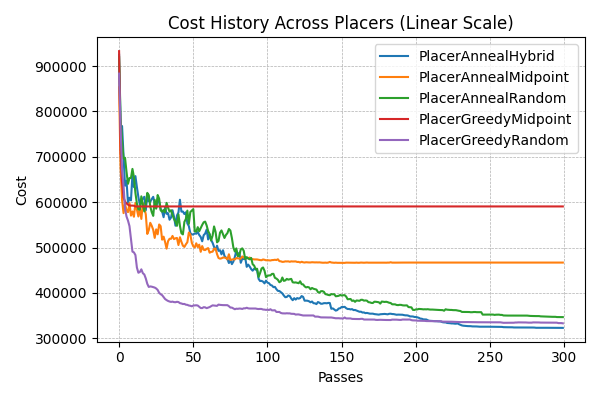
\includegraphics[width=\columnwidth]{figures/results/combined_cost_history_linear.png}
    \captionof{figure}{All placers overlaid}
    \label{fig:placers_overlay}
}


{
    \centering
    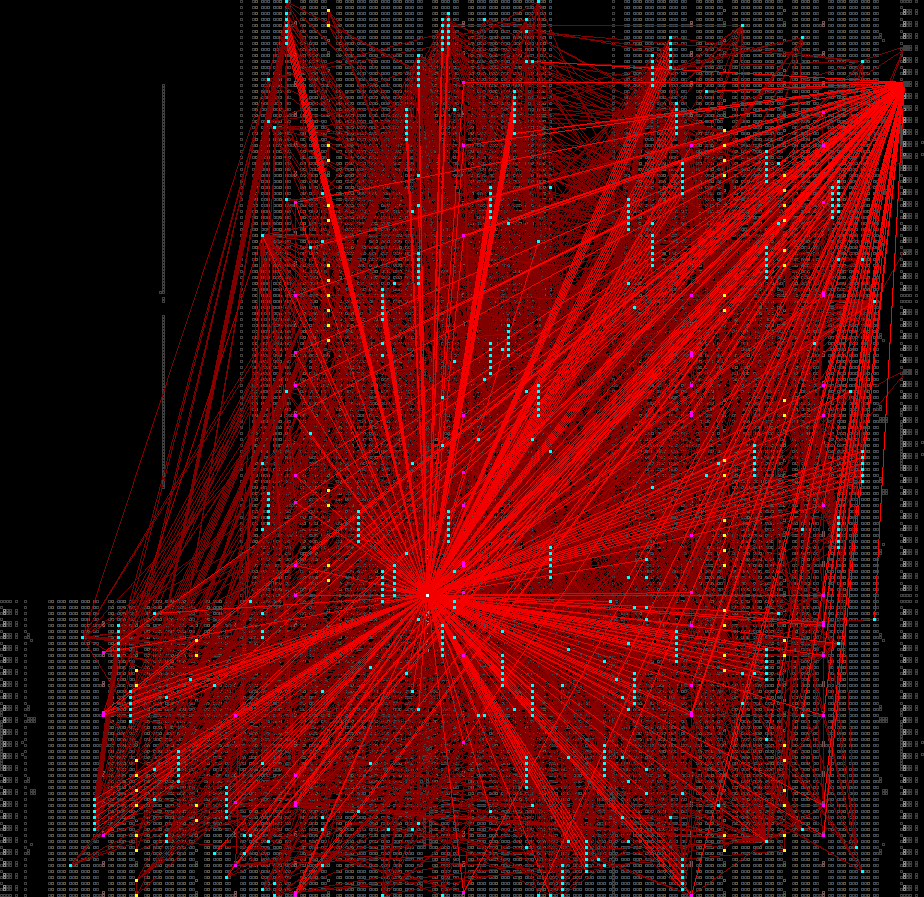
\includegraphics[valign=t, scale=0.13]{figures/results/PlacerGreedyRandom/random_placement.png}
    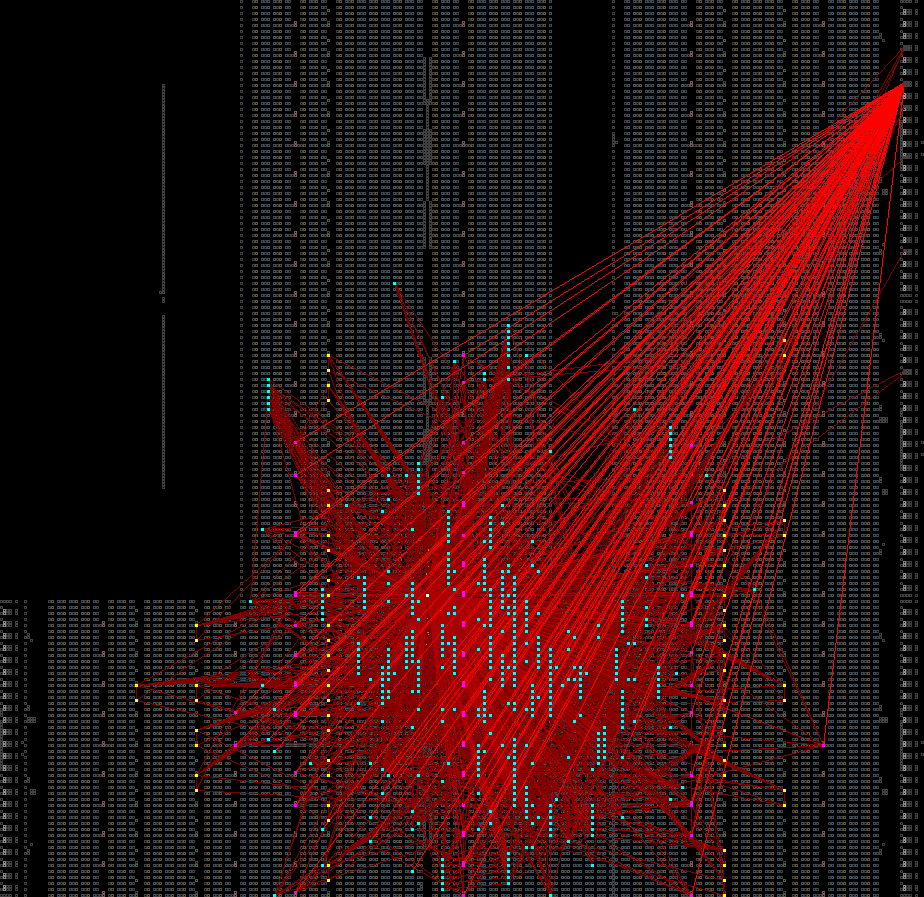
\includegraphics[valign=t, scale=0.13]{figures/results/PlacerGreedyRandom/00000010.png}
    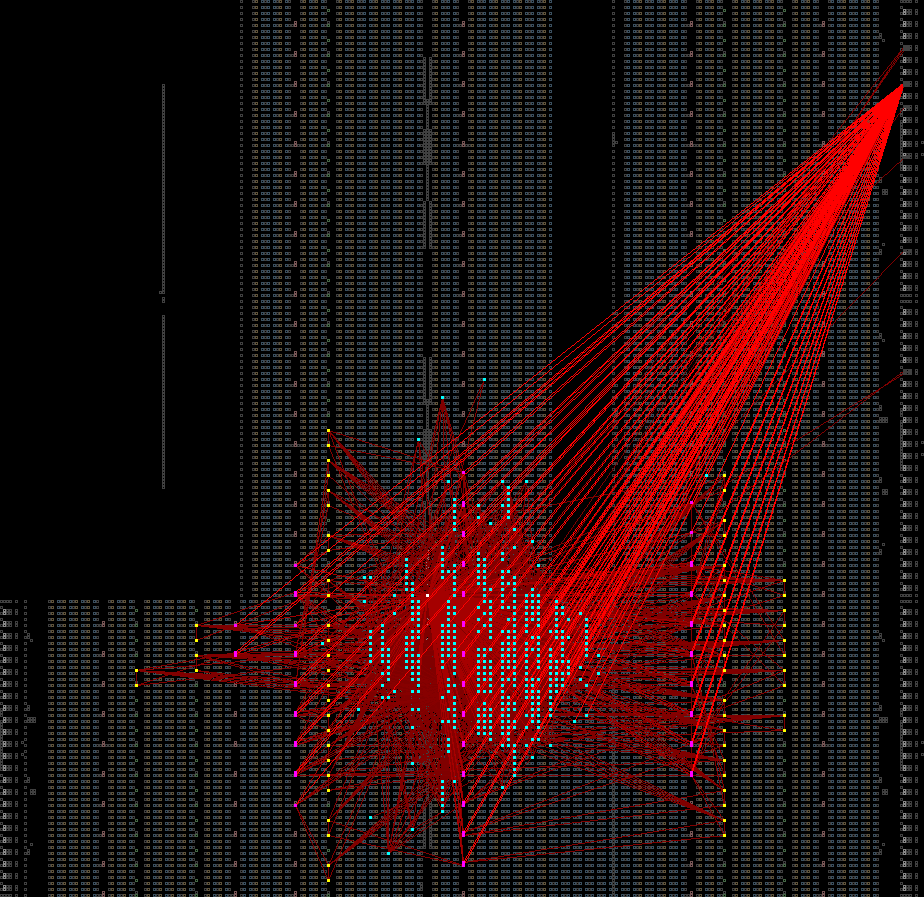
\includegraphics[valign=t, scale=0.13]{figures/results/PlacerGreedyRandom/00000100.png}
    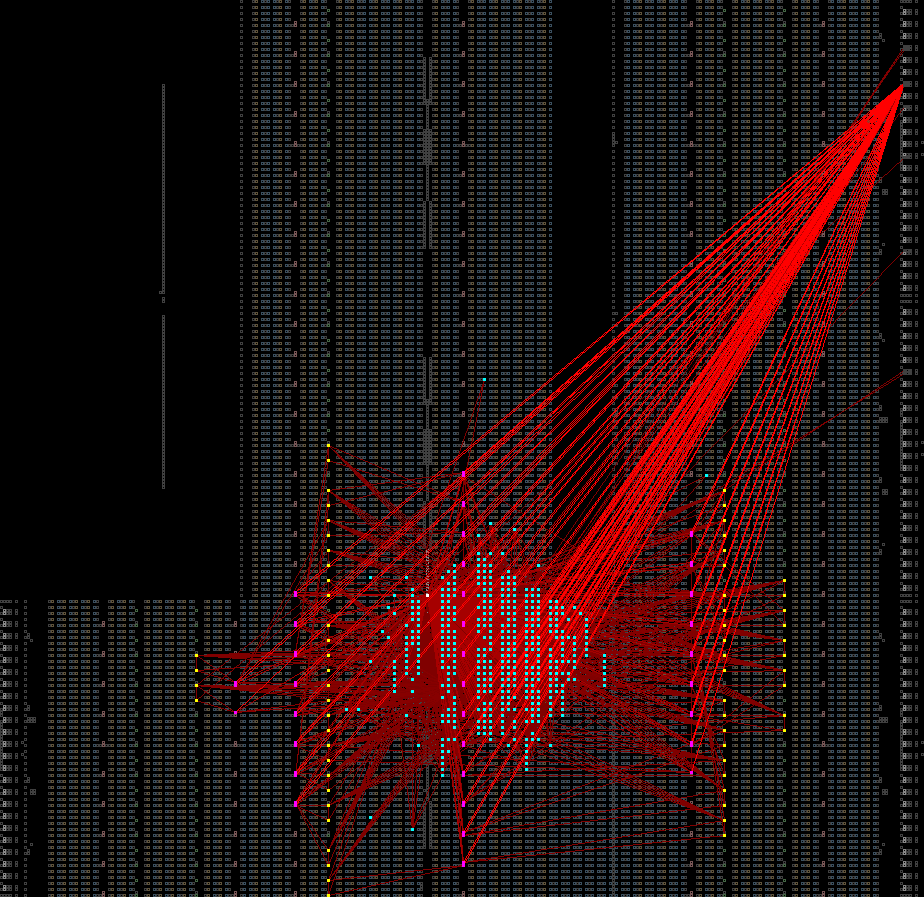
\includegraphics[valign=t, scale=0.13]{figures/results/PlacerGreedyRandom/00000299.png}
    \captionof{figure}{PlacerGreedyRandom}
    \label{fig:PGRSnapshots}
}

\columnbreak
{
    \centering
    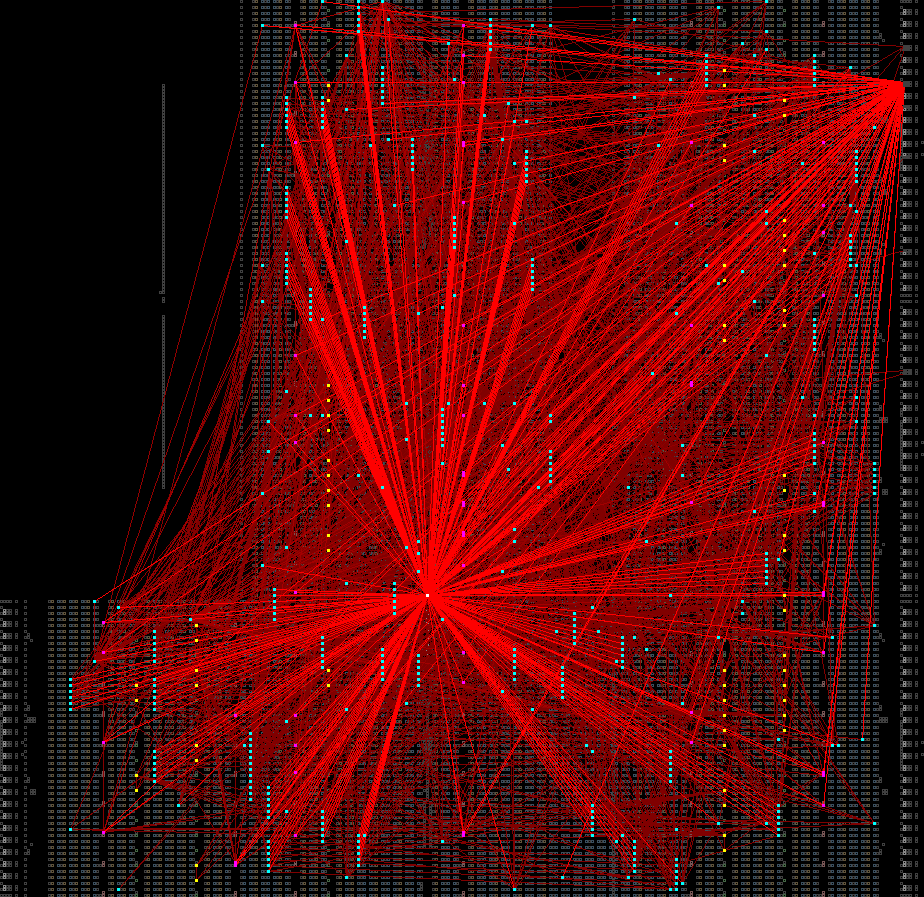
\includegraphics[valign=t, scale=0.13]{figures/results/PlacerGreedyMidpoint/random_placement.png}
    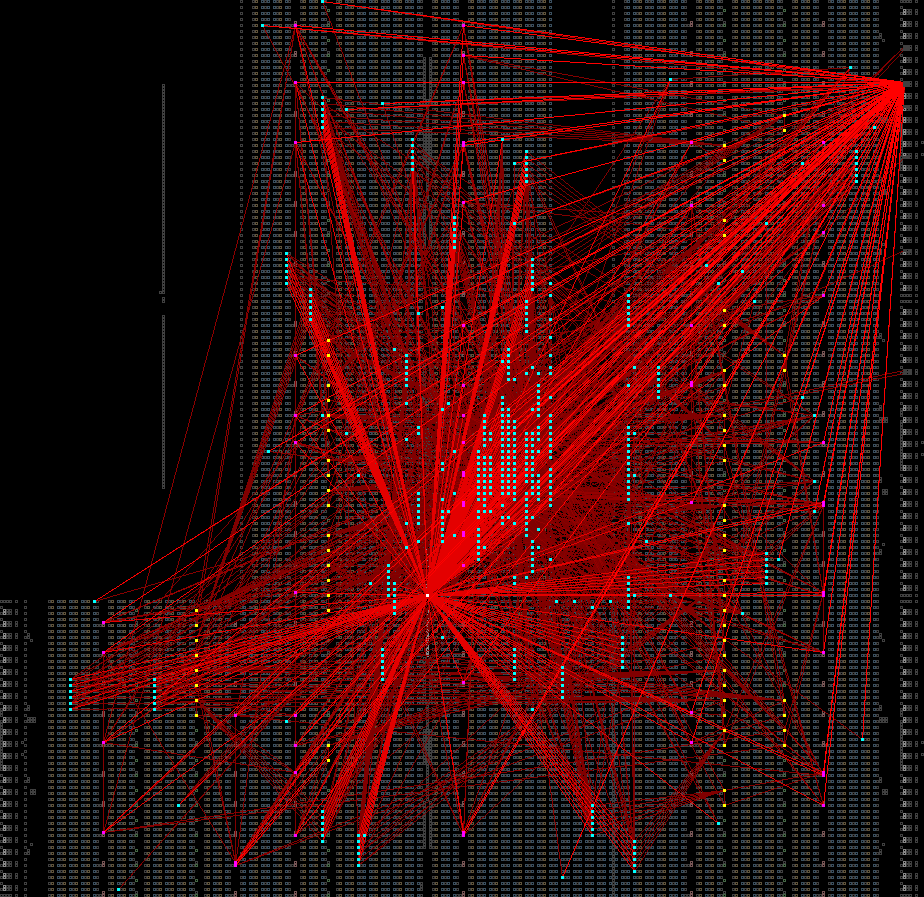
\includegraphics[valign=t, scale=0.13]{figures/results/PlacerGreedyMidpoint/00000010.png}
    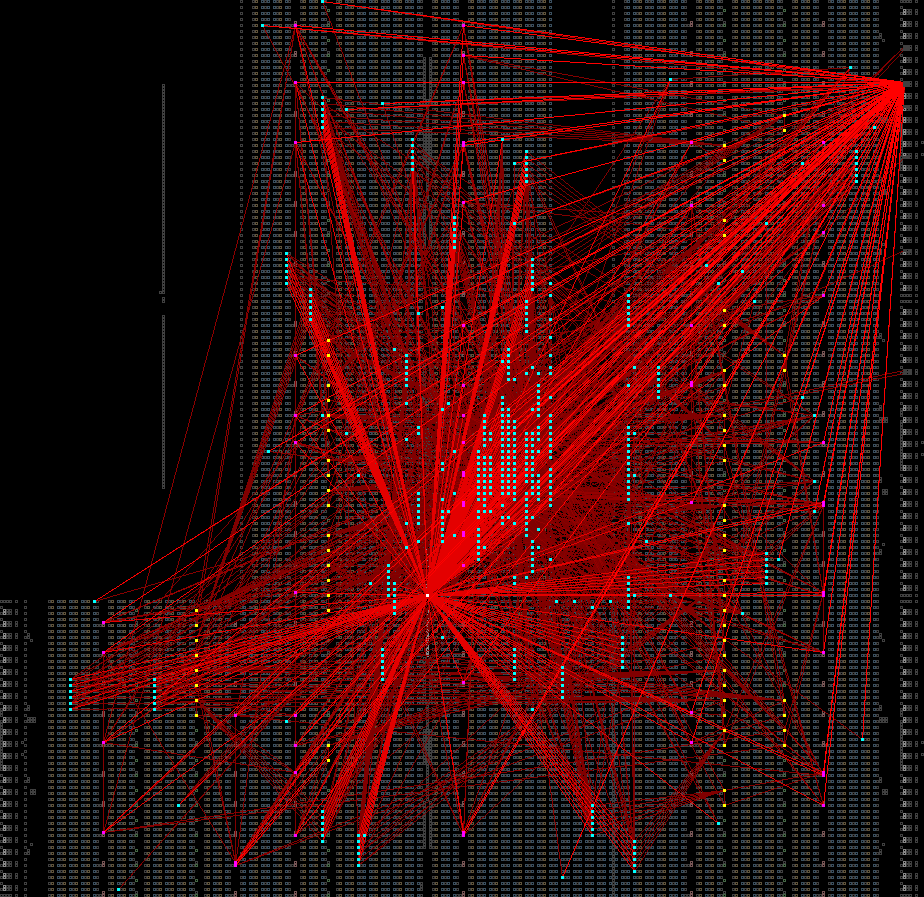
\includegraphics[valign=t, scale=0.13]{figures/results/PlacerGreedyMidpoint/00000100.png}
    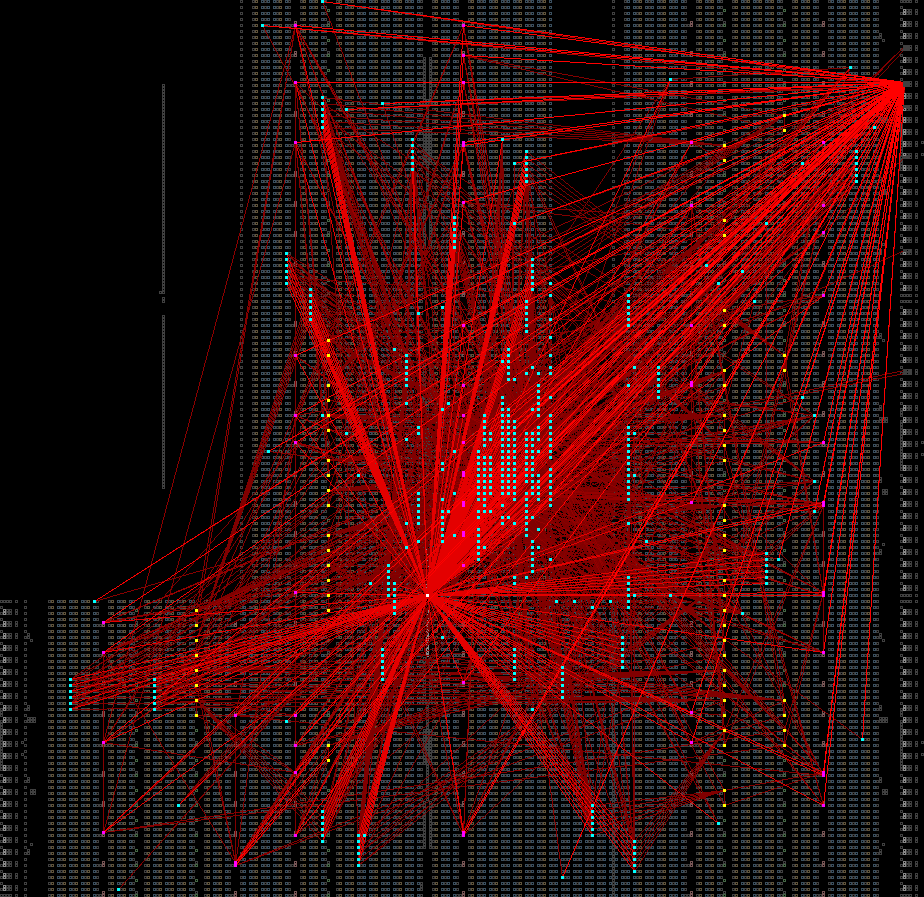
\includegraphics[valign=t, scale=0.13]{figures/results/PlacerGreedyMidpoint/00000299.png}
    \captionof{figure}{PlacerGreedyMidpoint}
    \label{fig:PGMSnapshots}
}
\vfill
{
    \centering
    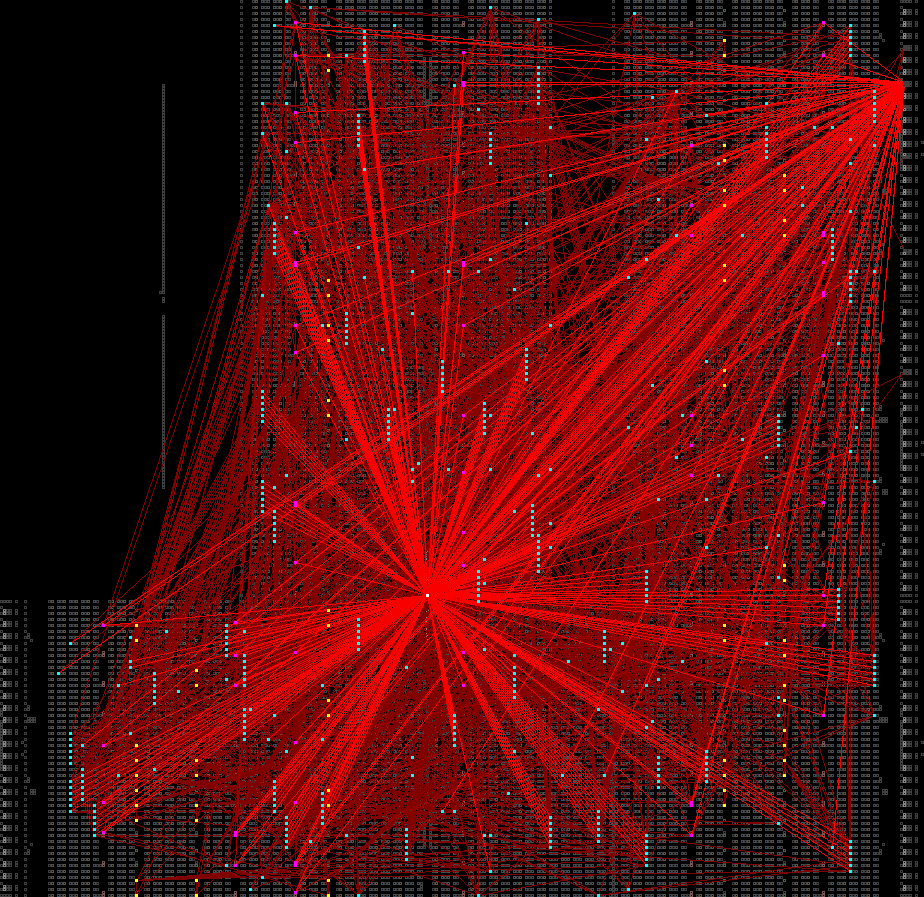
\includegraphics[valign=t, scale=0.13]{figures/results/PlacerAnnealRandom/random_placement.png}
    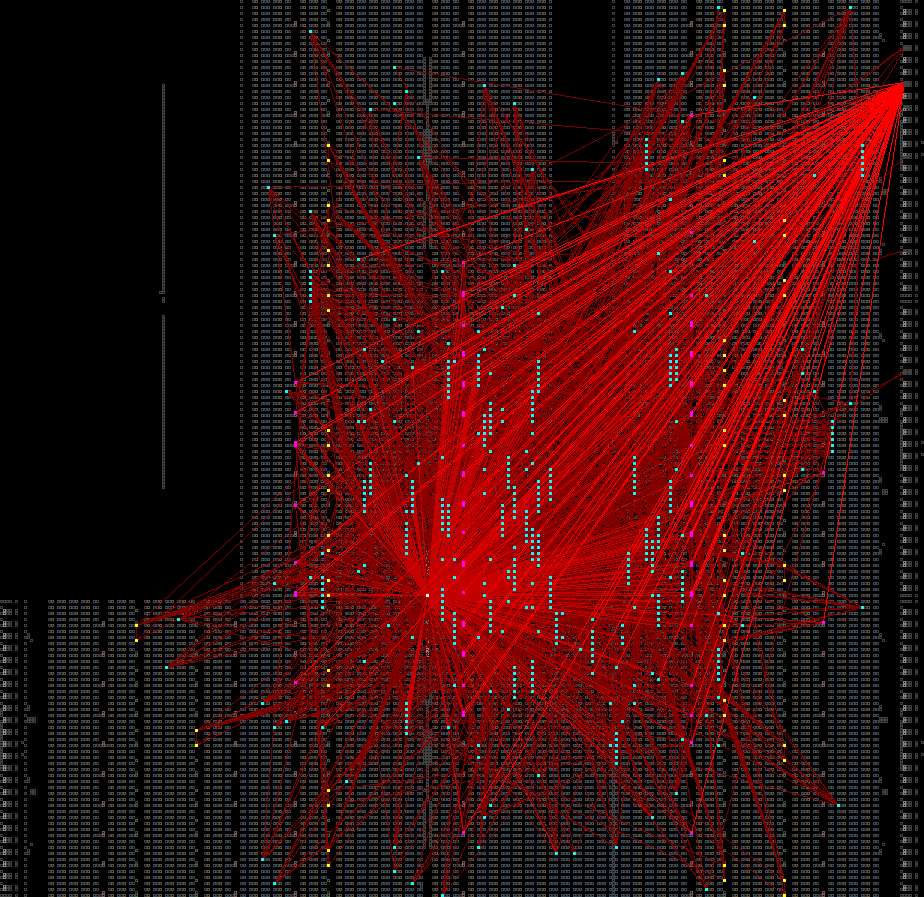
\includegraphics[valign=t, scale=0.13]{figures/results/PlacerAnnealRandom/00000010.png}
    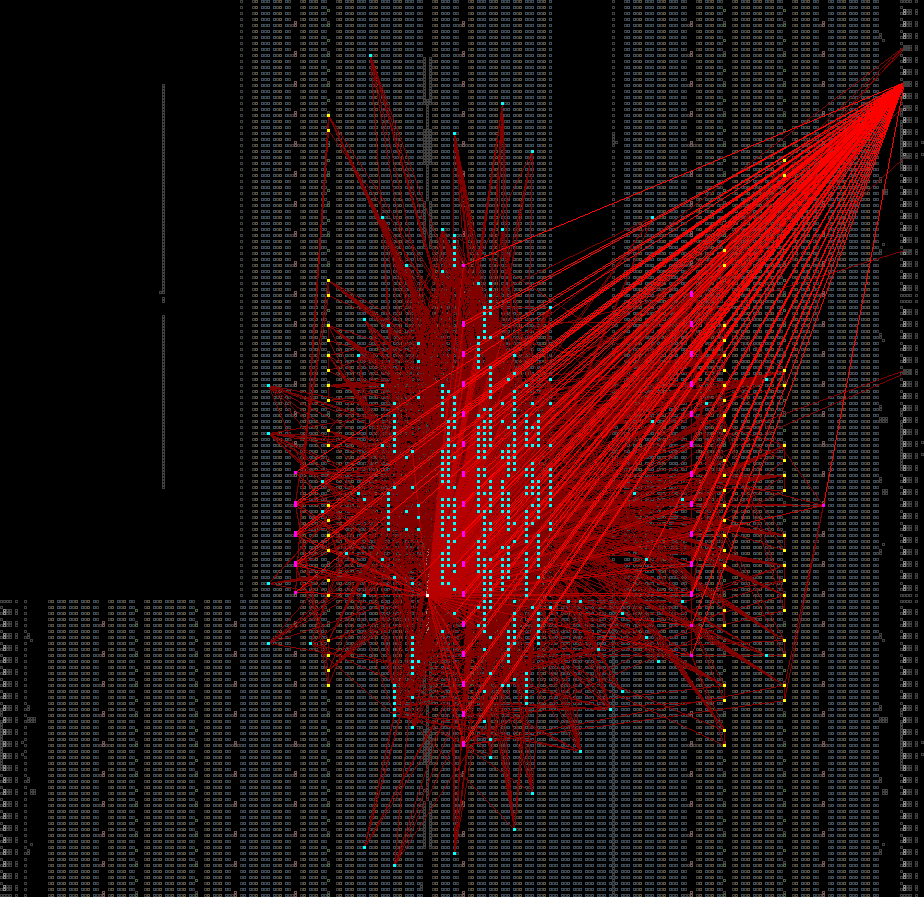
\includegraphics[valign=t, scale=0.13]{figures/results/PlacerAnnealRandom/00000100.png}
    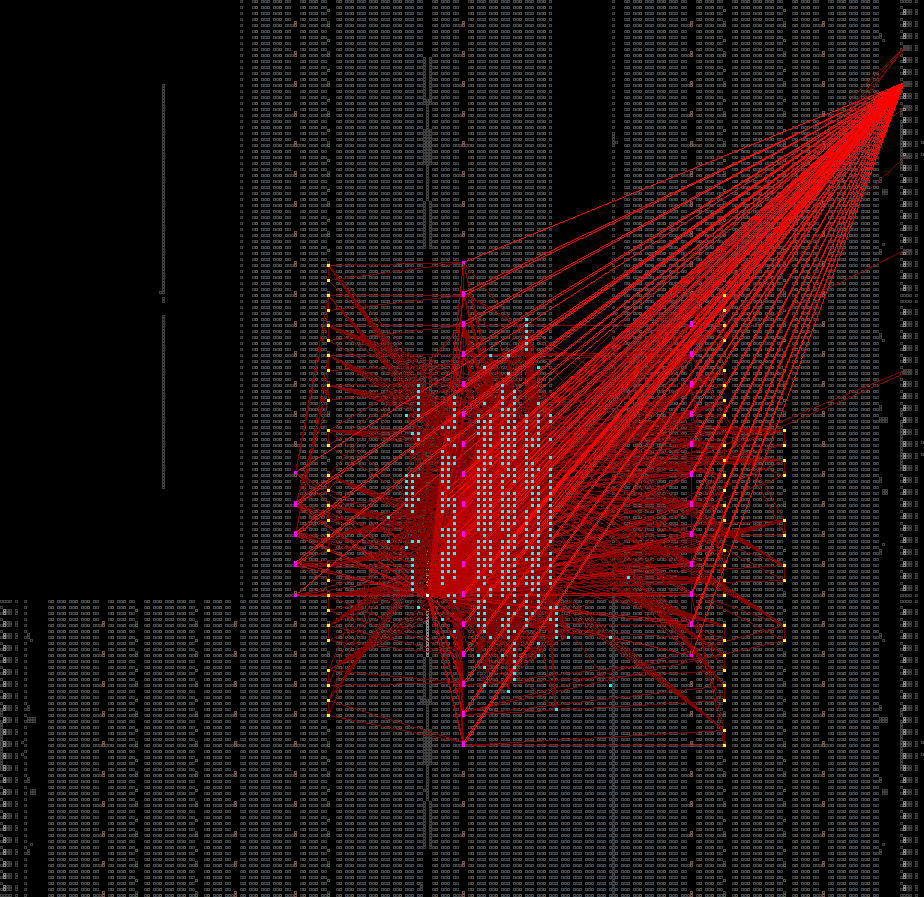
\includegraphics[valign=t, scale=0.13]{figures/results/PlacerAnnealRandom/00000299.png}
    \captionof{figure}{PlacerAnnealRandom}
    \label{fig:PARSnapshots}
}


\columnbreak
{
    \centering
    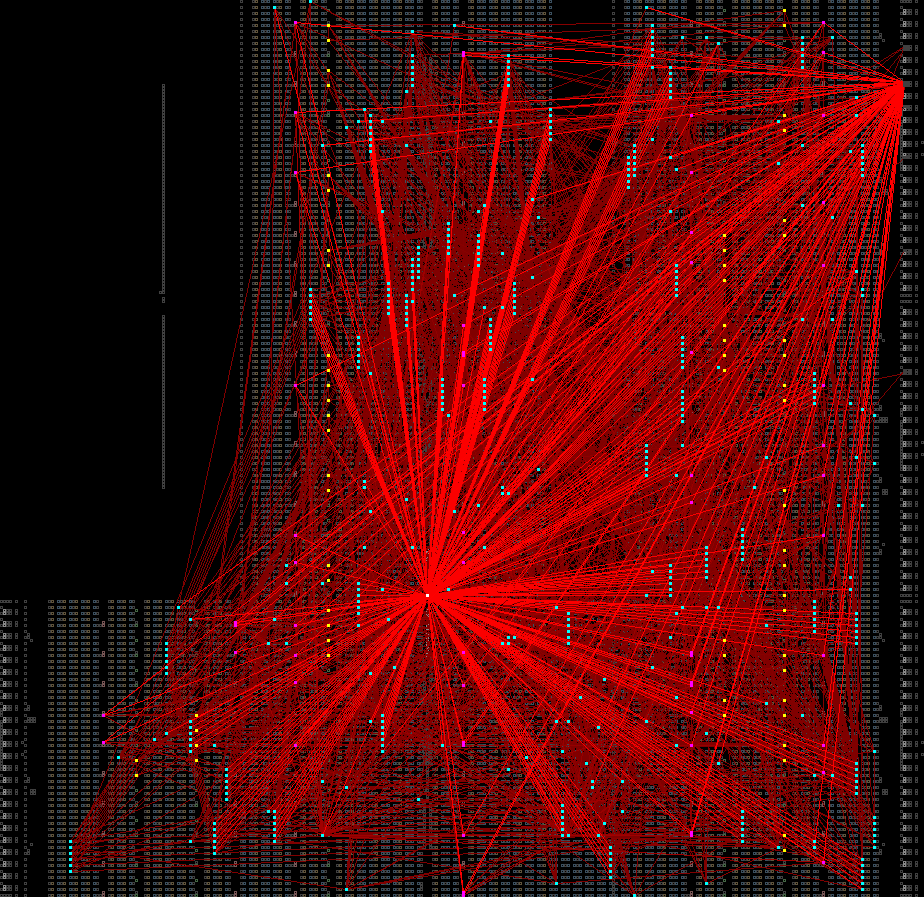
\includegraphics[valign=t, scale=0.13]{figures/results/PlacerAnnealMidpoint/random_placement.png}
    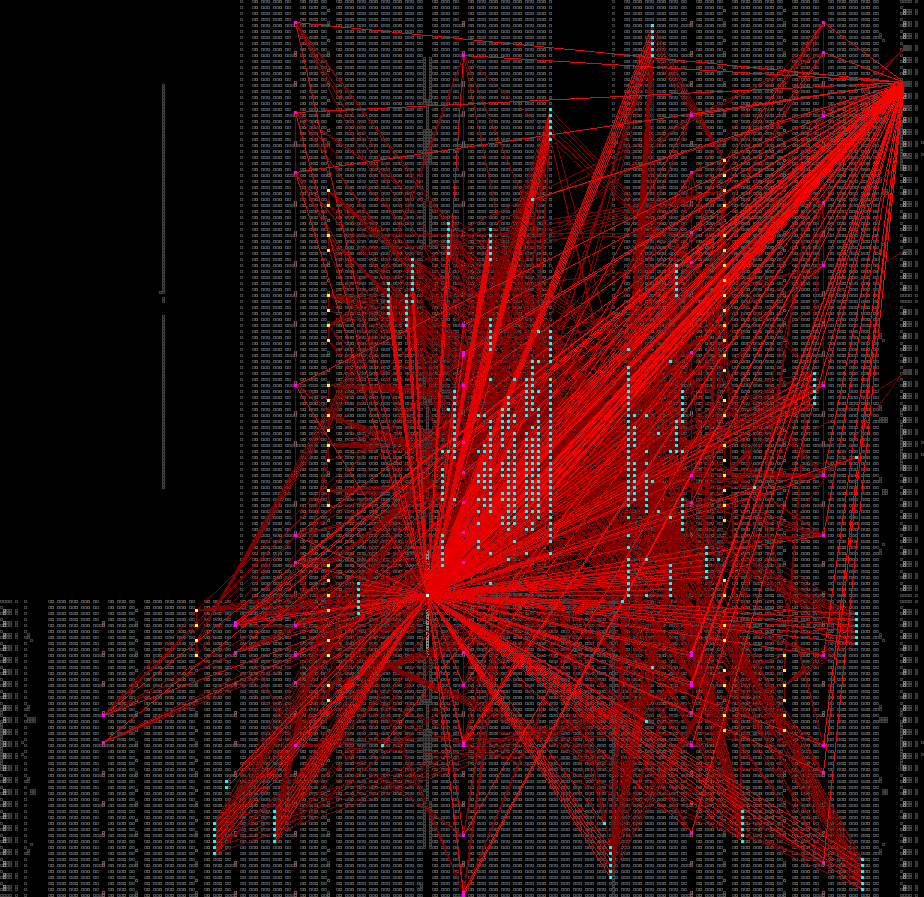
\includegraphics[valign=t, scale=0.13]{figures/results/PlacerAnnealMidpoint/00000010.png}
    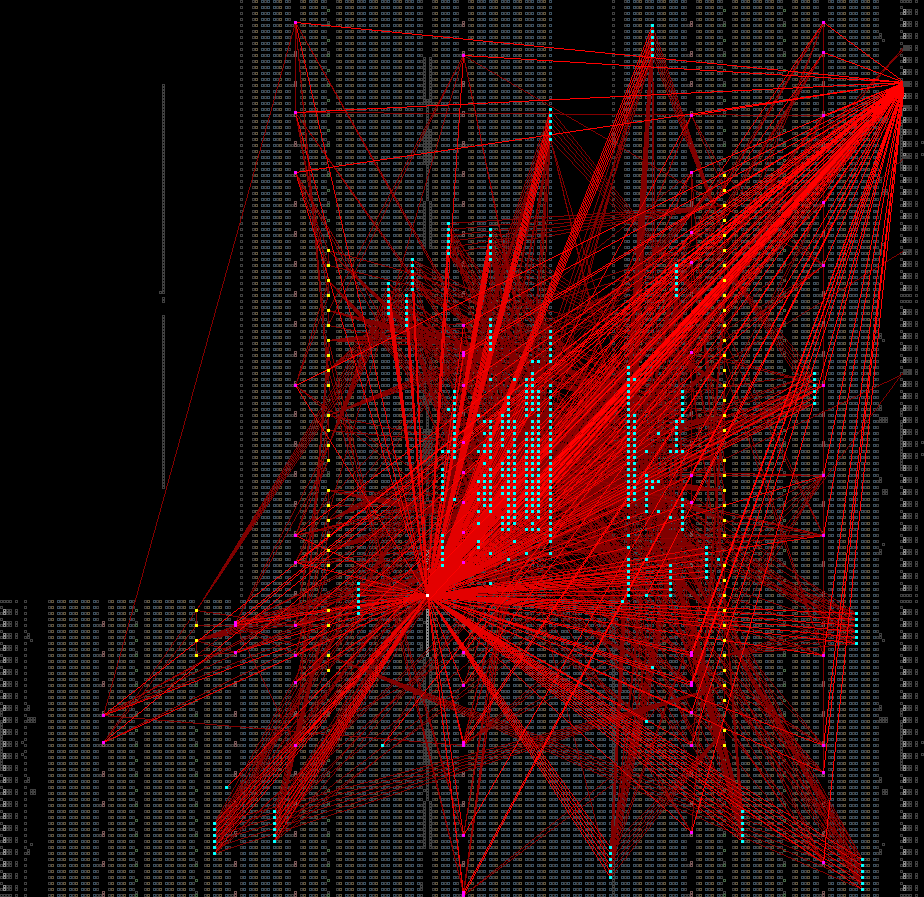
\includegraphics[valign=t, scale=0.13]{figures/results/PlacerAnnealMidpoint/00000100.png}
    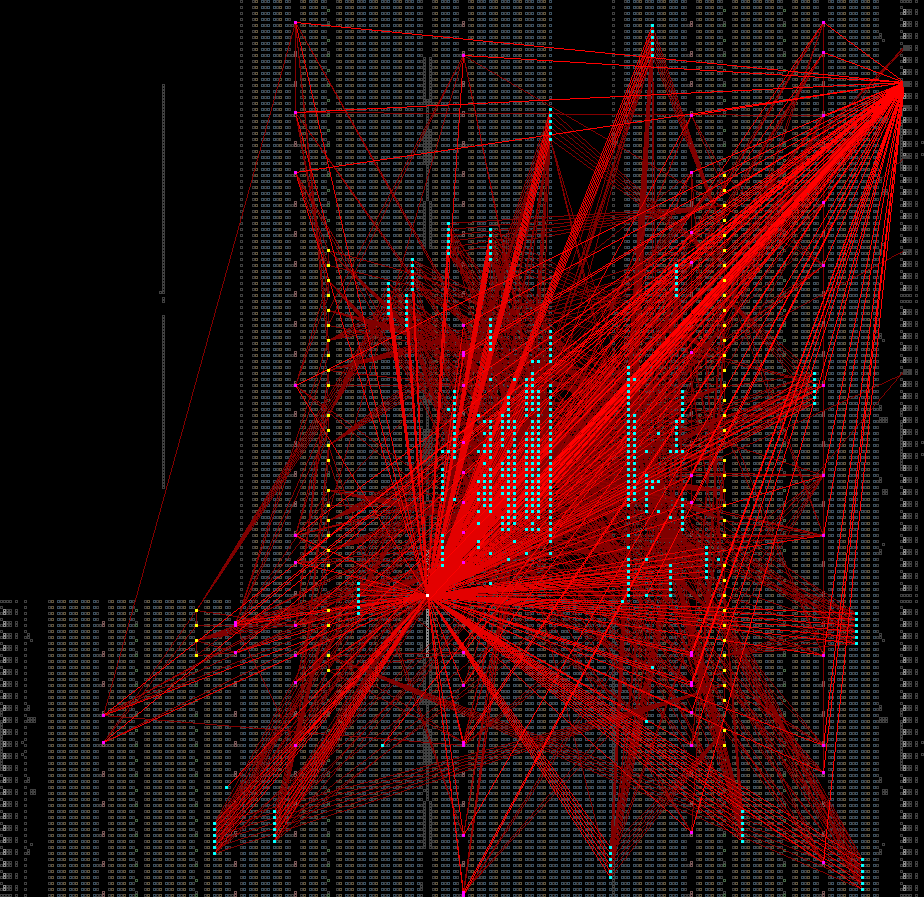
\includegraphics[valign=t, scale=0.13]{figures/results/PlacerAnnealMidpoint/00000299.png}
    \captionof{figure}{PlacerAnnealMidpoint}
    \label{fig:PAMSnapshots}
}
\vfill
{
    \centering
    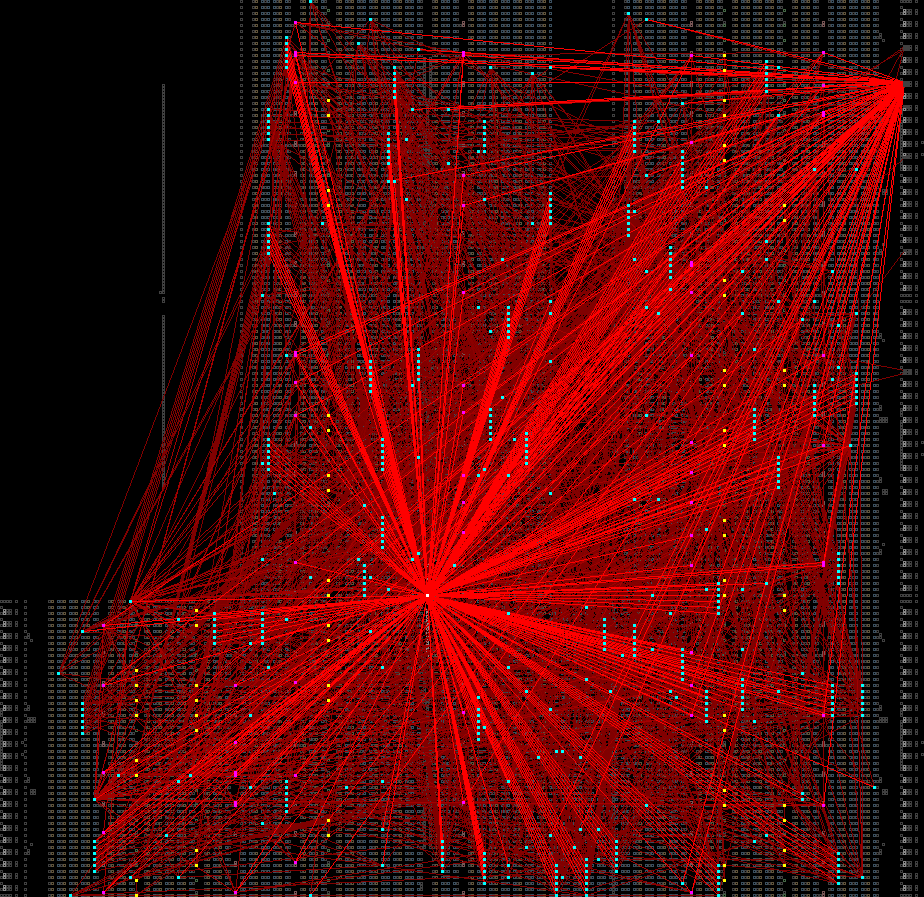
\includegraphics[valign=t, scale=0.13]{figures/results/PlacerAnnealHybrid/random_placement.png}
    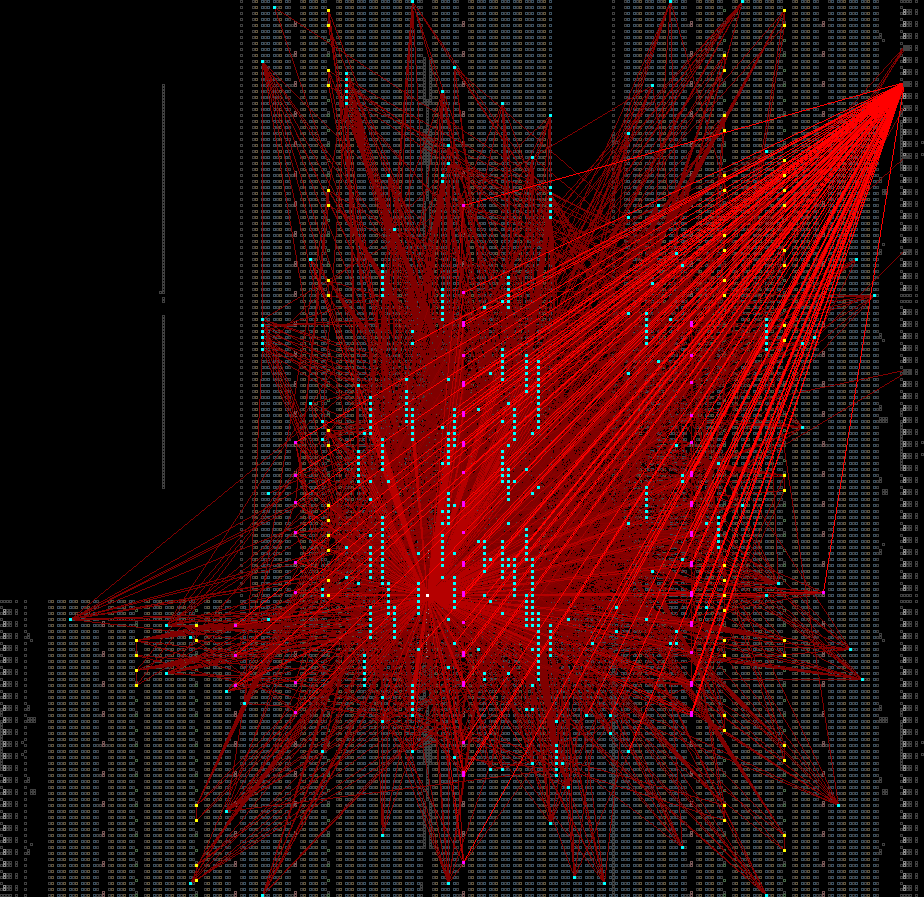
\includegraphics[valign=t, scale=0.13]{figures/results/PlacerAnnealHybrid/00000010.png}
    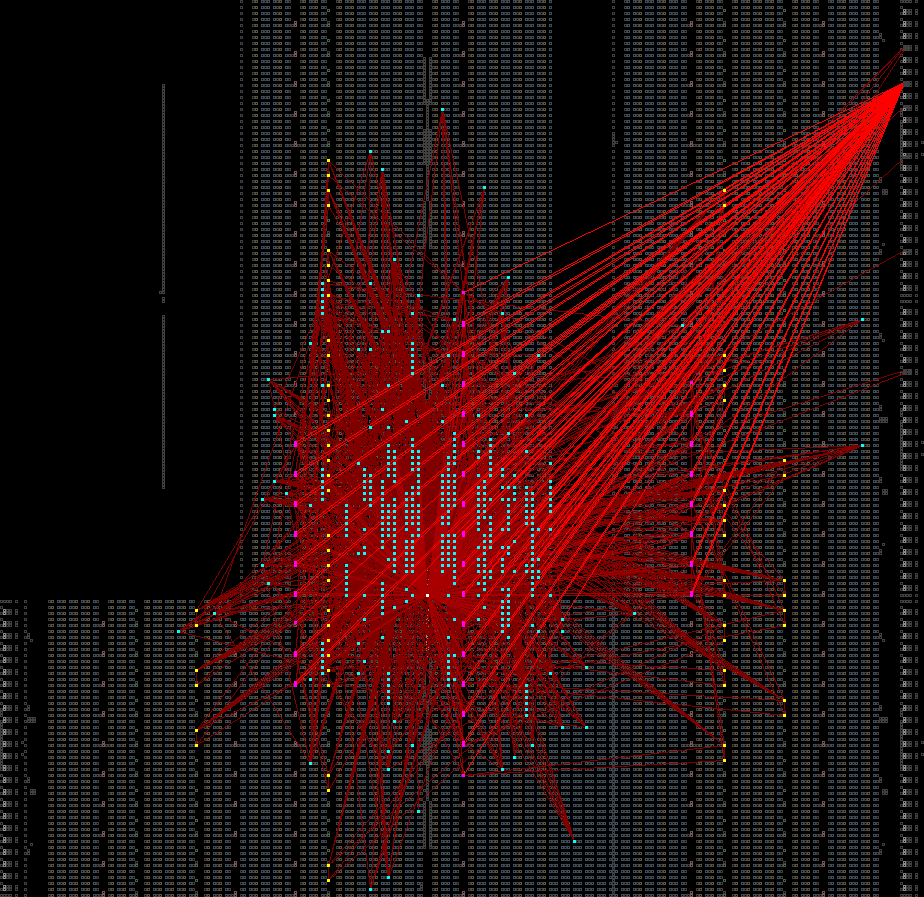
\includegraphics[valign=t, scale=0.13]{figures/results/PlacerAnnealHybrid/00000100.png}
    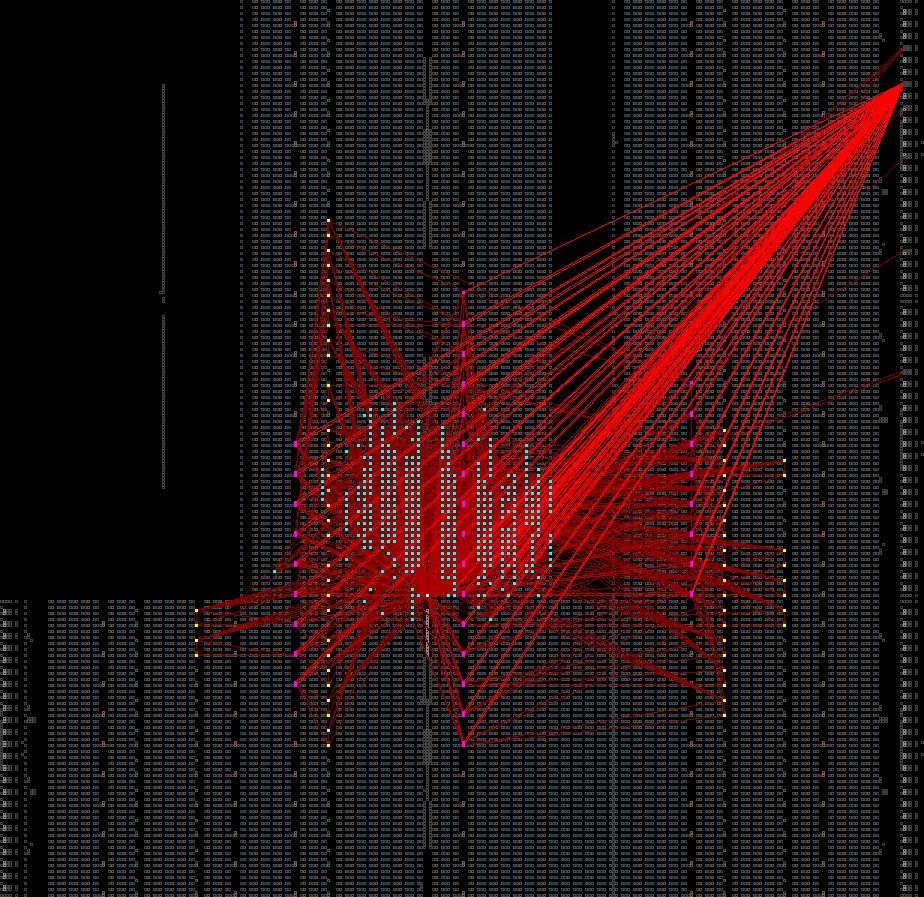
\includegraphics[valign=t, scale=0.13]{figures/results/PlacerAnnealHybrid/00000299.png}
    \captionof{figure}{PlacerAnnealHybrid}
    \label{fig:PAHSnapshots}
}


